\chapter{Serie}

\section{Serie numeriche}

Come nel campo dei reali, la serie numerica è scritta come $\sum_{i=0} ^{\infty} a_i$ con $a_i \in \C$; definita la successione delle somme parziali $S_n=\sum_{i=0} ^n a_i$, recuperiamo tutte le informazioni sulla convergenza già viste in altri ambiti:
\begin{teorema} (Criterio di convergenza secondo Cauchy)\\$S_n$ converge $\iff$ $S_n$ è di Cauchy, cioè se $\forall \epsilon >0 \exists N_{\epsilon}$ : $|S_{m+n} - s_m| < \epsilon$ $\forall m>N_{\epsilon}, \forall n>0$
\end{teorema}
La condizione che $|S_{m+n} - s_m| < \epsilon$ equivale a chiedere che $\left|\sum_{i=m+1} ^{m+n} a_i \right| < \epsilon$. \\Osserviamo che la condizione necessaria per la convergenza è che il termine generale (in modulo) vada a zero (questo perchè le formule sopra valgono $\forall m,n$). Oltretutto, abbiamo che $\left|\sum_{i=m+1} ^{m+n} a_i \right| \leq \sum_{i=m+1} ^{m+n} |a_i|$; definiamo quindi la \textbf{convergenza assoluta}, cioè la convergenza della serie dei moduli.
\begin{teorema}
Se una serie converge assolutamente, allora converge, cioè 
$$\sum |a_i|<\infty \implies \sum a_i<\infty$$
\end{teorema}
I criteri per la convergenza assoluta sono:
\begin{itemize}
\item Criterio del confronto:	$|a_i|<b_i$ $\forall i$ e $\sum b_i$ converge $\implies \sum a_i$ converge
\item Criterio della radice:		$\limsup_i \sqrt[i] {|a_i|} <1 \implies \sum a_i$ converge
\item Criterio del rapporto:		$\limsup_i \frac{a_{i+1}}{a_i}<1 \implies \sum a_i$ converge
\end{itemize}
	Sia nel caso del criterio del confronto sia nel caso del criterio della radice, nel momento in cui esiste il limite normale non dobbiamo scomodale il lim sup, ma possiamo ricorrere al limite semplice.

\section{Serie geometrica}

La serie geometrica è una serie della forma $\sum_{n=0} ^{\infty} z^n$; di questa serie sappiamo calcolare il valore effettivo della somma; infatti si ha che $S_n=1+z+z^2+z^3+ \dots +z^n$ e $S_{n+1}=S_n + z^{n+1}$; quindi si ha che $z \, S_n=S_{n+1} -1$ e, sostituendo le relazioni precedentemente ricavate, si ottiene che $S_n=\frac{1-z^{n+1}}{1-z}$. Da quì è facile osservare che la convergenza di $S_n$ dipende dal valore di z, cioè che $S_n$ converge se $|z|<1$; valutando la serie per $n \to \infty$ si ha che $\sum_{n=0} ^{\infty} z^n=\frac{1}{1-z}$, con $|z|<1$.
\\Esempi:
\begin{itemize}
\item $e^z =e^x e^{iy}=e^x (cos(y)+i sen(y))$ \\$e^z=\sum \frac{z^n}{n!}$ converge assolutamente su $\C$
\item $\sum \frac{1}{n^z} = \zeta(z)$: la funzione Zeta di Riemann converge se $Re(z)>1$
\end{itemize}

\section{Serie di funzioni}

Consideriamo la successione di funzioni $\{f_k\}$ con $f_k:E \to \C$ (dove E non deve per forza essere un sottoinsieme di $\C$); cosa sono la convergenza puntuale e la convergenza uniforme? \\La convergenza puntuale in un punto $p \in E$ si rivela essere la solita condizione di Cauchy:

$$\forall \epsilon >0 \, \, \exists N_{\epsilon, p} \text{ : } |f_n(p) -f_m(p)| < \epsilon \, \, \forall n,m>N_{\epsilon, p}$$ 
Per quanto riguarda la convergenza uniforme, invece, l'indice N non dipende dal punto p:
$$\forall \epsilon >0 \,\, \forall p \in E \, \, \exists N_{\epsilon} \text{ : } |f_n(p) -f_m(p)| < \epsilon \, \, \forall n,m>N_{\epsilon}$$
Consideriamo ora la successione delle somme parziali $S_n(p)=\sum_{k=0} ^{\infty} f_k(p)$; $S_n$ converge uniformemente su E se $\forall \epsilon >0 \, \, \forall p \in E \, \, \exists N_{\epsilon}$ : $|\sum_{k=m+1} ^{m+n} f_k(p)| < \epsilon$ $\forall m>N_{\epsilon}, \forall n>0$.
\\Vediamo ora una condizione sufficiente per la convergenza uniforme:
\begin{teorema} (Criterio M di Weierstrass)\\
Se $\exists b_k>0$ : $|f_k(p)|<b_k$ $\forall p \in E$, con $\sum_k b_k$ convergente $\implies \sum_k f_k(p)$ converge.
\end{teorema}
D'ora in avanti, parleremo di funzioni in cui il dominio $D \in \C$, cioè funzioni $f_k:D \subset \C \to \C$.
\begin{teorema}
Sia data una serie $\sum_{k=0} ^{\infty} f_k(z)$ convergente su $D \in \C$ e sia $\gamma$ un cammino differenziabile a tratti in D. Allora 
$$\int_{\gamma} \sum_{k=0} ^{\infty} f_k(z) dz=\sum_{k=0} ^{\infty} \int_{\gamma} f_k(z) dz$$
\end{teorema}

\begin{proof}
Definiamo la funzione $S_n(z)=\sum_{k=0} ^n f_k(z)$; sappiamo che ogni $S_n$ è continua, perchè somma di funzioni continue. Oltre ciò, ho (per ipotesi) che $S_n$ converge uniformemente su D ad un limite $S$, e in particolare lo farà sul compatto $\gamma$. \footnote{Parliamo di $\gamma$ come compatto perchè il cammino $\gamma:[a;b] \to \C$ parametrizzato rappresenta un compatto.} Allora $S$ è continua su $\gamma$, cioè esiste $\int_{\gamma} S(z) dz
$. \\Calcoliamo $\left|\sum_{k=0} ^n \int_{\gamma} f_k(z)dz - \int_{\gamma} \sum_{k=0} ^n f_k(z)dz \right| =$\footnote{Dato che abbiamo una somma finita, possiamo portare il simbolo di sommatoria dentro il primo integrale.}$\left|\int_{\gamma} [S_n(z)-S(z)]dz \right| \leq L[\gamma] \epsilon$; infatti si ha che $\forall \epsilon >0$ $\exists N$ : $|S_n-S|<\epsilon$ $\forall n>N$. \\Dato che vale per ogni $\epsilon$, si ha che $\sum_{k=0} ^n \int_{\gamma} f_k(z)dz=\int_{\gamma} \sum_{k=0} ^n f_k(z)dz$.

\end{proof}
Definiamo ora la \textbf{convergenza normale} di una serie di funzioni complesse:
\begin{definizione}
Una serie di funzioni $f_k:D \subset \C \to \C$ converge normalmente se:
\begin{itemize}
\item Converge puntualmente $\forall p \in D$
\item $\forall p$ esiste un disco chiuso dove la serie converge uniformemente
\end{itemize}
\end{definizione}
Attraverso la convergenza normale possiamo dare una dimostrazione alternativa del teorema precedente.

\section{Serie di potenze}

Una serie di potenze è una serie di funzioni della forma:

\begin{equation}
\sum_{k=0} ^{\infty} c_k (z-a)^k, \, c_k \in \C
\end{equation}
Il punto a è detto \textbf{centro della serie}.

\begin{teorema} (di Abel-Weierstrass)
\\Se la serie di potenze $\sum_{k=0} ^{\infty} c_k (z-a)^k$ converge per $z=z_0$, allora:

\begin{enumerate}
\item La serie converge assolutamente $\forall z$ nel disco aperto $|z-a|<|z_0-a|$
\item La serie converge uniformemente su ogni disco chiuso di raggio $|z_0-a|(1- \eta)$, con $\eta \in (0;1)$
\end{enumerate}
\end{teorema}
\begin{proof}
Dimostriamo i due punti separatamente:
\begin{enumerate}
\item Dato che la serie converge in $z_0$, si ha che $\exists N$ : $|c_k||z_0-a|^k<1$ $\forall k>N$. Da questo, ricaviamo che $|c_k| < \frac{1}{|z_0-a|^k}$; quindi, possiamo scrivere che $|c_k(z-a)^k|= |c_k||z-a|^k<\left|\frac{z-a}{z_0-a}\right|^k$. Allora si ha che $\sum_{k=0} ^{\infty} c_k (z-a)^k$ converge assolutamente, poichè si ha che $\sum_{k=0} ^{\infty} |c_k (z-a)^k|<$ $<\sum_{k=0} ^{\infty} \left|\frac{z-a}{z_0-a}\right|^k$, la quale converge purchè $\left|\frac{z-a}{z_0-a}\right|<1$, cioè $|z-a|<|z_0-a|$.
\item Poniamo su $z$ la condizione che $|z-a|\leq |z_0-a|(1-\eta)$; per quanto visto nel punto precedente, abbiamo visto che esiste un $N$ tale che $\forall k>N$ si ha che $\left|c_k(z-a)^k\right| \leq \frac{1}{|z_0-a|^k} |z-a|^k \leq$ $\leq  \frac{1}{|z_0-a|^k} |z_0-a|^k (1-\eta)^k=(1-\eta)^k$ e si ha che $\sum_k (1-\eta)^k$ converge.
\end{enumerate}

\end{proof}
Cosa può succedere alla convergenza di una serie di potenze? Grazie a questo teorema, possiamo esprimere tre possibili casi:
\begin{itemize}
\item La serie converge solo per $z=a$
\item La serie converge su tutto $\C$ (o comunque in tutto l'insieme di definizione)
\item La serie non converge ovunque, ma converge in almeno un punto $z_0 \neq a$
\end{itemize}
In quest'ultimo caso, andiamo a definire una zona del piano complesso in cui la serie converge; tale area è rappresentata dal raggio di convergenza (che, nel caso in cui la serie non converga ovunque, è finito).

\section{Raggio di convergenza di una serie}

\begin{teorema} (Criterio di Cauchy-Hadamard)\\
La serie $\sum_k |c_k(z-a)^k|$ converge se $\limsup_k \sqrt[k]{|c_k(z-a)^k|} <1$.
\end{teorema}
Otteniamo che $\frac{1}{|z-a|} > \limsup_k \sqrt[k]{|c_k|} \equiv \frac{1}{R}$; quindi si ha $|z-a|=R$ e $\limsup_k \sqrt[k]{|c_k|} = R^{-1}$.
\begin{teorema}	

Sia $f$ una funzione olomorfa su D. Sia $D(a,r)$ un disco di raggio r centrato in a, contenuto in $D$ con contorno $C(a,r)$ \footnote{Circonferenza centrata in a e di raggio r.}. Si ha che:
$$\forall z \in D(a,r)\text{ }f(z)=\sum_{k=0} ^{\infty} c_k (z-a)^k\text{, con }c_K= \int_{C(a,r)} \frac{f(z)}{(z-a)^{k+1}} \frac{dz}{2 i \pi}$$
cioè, per ogni punto z appartenente al disco $D(a,r)$ la funzione $f$ può essere riscritta sottoforma di serie di potenze, co n i coefficienti $c_k$ ben definiti.
\end{teorema}
\begin{proof}
Partiamo dalla formula integrale di Cauchy applicata a $f(z)$; abbiamo che $f(z)=\int_{C(a,r)} \frac{f(s)}{s-z} \frac{ds}{2 i \pi}$. \\Riscriviamo $\frac{1}{s-z}$ come $\frac{1}{(s-a)-(z-a)}=\frac{1}{s-a} \frac{1}{1-\frac{z-a}{s-a}}= \sum_{n=0} ^{\infty} (\frac{z-a}{s-a})^n$; sostituiamo la serie all'interno dell'integrale, e otteniamo che:
$$f(z)=\int_{C(a,r)} \frac{f(s)}{s-a} \sum_{n=0} ^{\infty} \left(\frac{z-a}{s-a}\right)^n \frac{ds}{2 i \pi}=\footnote{Dato che la serie converge uniformemente, possiamo portare la sommatoria fuori dall'integrale.} \sum_{n=0} ^{\infty} (z-a)^n \int_{C(a,r)} a\frac{f(s)}{(s-a)^{n+1}} \frac{ds}{2 i \pi}$$
che è la costruzione dettata dal teorema.
 
 \end{proof}

\subsection{Prodotto di cauchy di due serie di potenze con centro in a=0}

Siano date due serie $\sum_{k=0} ^{\infty} a_k$ e $\sum_{l=0} ^{\infty} c_l$; definiamo il \textbf{prodotto di Cauchy} delle due serie è la serie $\sum_{m=0} ^{\infty} \sum_{k=0} ^m a_k c_{m-k}$. \\Similmente, date due serie di potenze $\sum_{k=0} ^{\infty} a_k z^k$ e $\sum_{l=0} ^{\infty} c_l z^l$, il prodotto di Cauchy delle due serie di potenze è $\sum_{m=0} ^{\infty} z^m \sum_{k=0} ^m a_k c_{m-k}$. 

Notiamo che se delle due serie una converge assolutamente e l'altra converge semplicemente (o puntualmente), allora il prodotto di Cauchy converge semplicemente (o puntualmente), mentre se entrambe convergono assolutamente allora anche il prodotto di Cauchy converge assolutamente.
\\
Quando abbiamo una singolarità e vogliamo sviluppare la funzione in serie di potenze, tale serie convergerà in un disco di raggio al più uguale al minimo fra le distanze fra il centro della serie e i punti in cui ho singolarità.
\\
Esempi:
\begin{itemize}
\item Sia data la funzione $f(z)=\frac{1}{(z-1)(z-3)}$; gli sviluppi in serie centrati nei punti A e C convergono nei due dischi riportati.
\begin{figure}[h!]
  \centering
    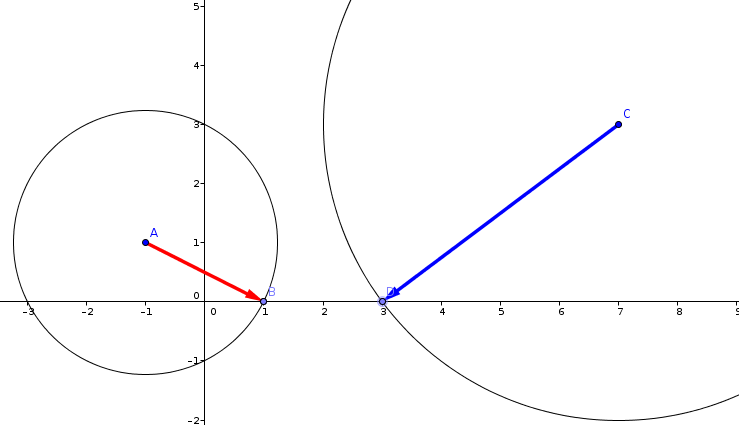
\includegraphics[width=0.5\textwidth]{immagini/frazione-polinomio-2.png}
\end{figure}
\item Sia data la funzione logaritmo principale; i dischi di convergenza delle serie risultano essere delle due tipologie riportate in figura:
\begin{figure}[h!]
  \centering
    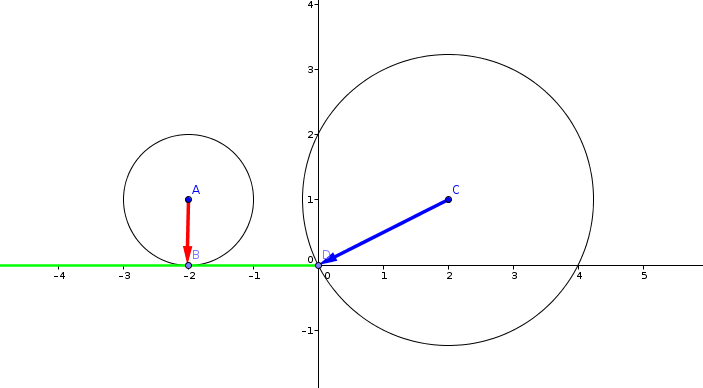
\includegraphics[width=0.5\textwidth]{immagini/logaritmo-2.png}
\end{figure}
\end{itemize}
Vediamo ora in che rapporto stanno la derivata di una serie e la serie di partenza:
\begin{teorema}
La serie $S(z)=\sum_{n=0} ^{\infty} c_n (z-a)^n$ e la sua serie derivata $S'(z)=\sum_{n=1} ^{\infty} n c_n (z-a)^{n-1}$ hanno lo stesso raggio di convergenza, cioè convegono sullo stesso disco aperto.
\end{teorema}

Sia $f$ una funzione olomorfa in un dominio $\mathbb{D}$, con $f(z)=\sum_{n=0} ^{\infty} c_n (z-a)^n$ nel disco aperto $D(a,r) \subset \mathbb{D}$. Abbiamo visto che i coefficienti $c_n$ sono da $\oint_{C(a,r)} \frac{f(z)}{(z-a)^{n+1}} \frac{dz}{2 i \pi}$; oltretutto, per $z \in \mathbb{D}$, grazie alla formula integrale di Cauchy abbiamo che:
$$f(z)=\oint_{C(a,r)} \frac{f(z')}{z'-z} \frac{dz'}{2 i \pi}$$
che, valutato in $z=a$, ci dà $c_0$, cioè $c_0=f(a)$. 
\clearpage
Similmente, abbiamo che
$$f'(z)=\oint_{C(a,r)} \frac{f(z')}{(z-z')^1} \frac{dz'}{2 i \pi}$$
che, valutato in $z=a$, ci dà $c_1=f'(a)$. Procedendo in tale maniera, otteniamo che i coefficienti $c_n$ sono dati dalla formula:
$$c_n=\frac{f^{(n)}(a)}{n!}=\oint_{C(a,r)} \frac{f(z)}{z-a} \frac{dz}{2 i \pi}$$

\section{Polinomi di Hermite}

Sia $H(z,x)=e^{-z^2+2xz}$ una funzione intera per ogni $x \in \R$ (ma lo è anche per $x \in \C$). Prendiamone lo sviluppo in serie di potenze centrato in $z=0$:
\begin{equation}
H(0,x)= \sum_{n=0} ^{\infty} z^n \frac{H_n(x)}{n!}
\end{equation}
Viene definita un'intera famiglia di funzioni $H_n$ a partire da un'unica funzione $H(z,x)$; tale funzione è detta \textbf{funzione generatrice} (dei \textbf{polinomi di hermite}). Grazie a quanto visto per le serie di potenze, dato che i vari $ \frac{H_n(x)}{n!}$ rappresentano i coefficienti $c_n$ della serie, ricaviamo che 
$$\frac{H_n(x)}{n!}=\oint \frac{H(z,x)}{z^{n+1}} \frac{dz}{2 i \pi}=\oint \frac{e^{-z^2+2xz}}{z^{n+1}} \frac{dz}{2 i \pi}$$
Sviluppando in serie l'esponenziale, otteniamo che 
$$ \frac{H_n(x)}{n!}=\sum_{l=0} ^{\infty} \frac{(2x)^l}{l!} \oint e^{-z^2} z^{l-n-1} \frac{dz}{2 i \pi}$$
Se $l-n-1 \geq 0$, allora $e^{-z^2} z^{l-n-1}$ è una funzione intera e quindi, per il teorema di Cauchy, l'integrale si annulla; questo fa sì che la somma sulle $l$ diventi una somma finita, poichè l'integrale è nullo se $l \geq n+1$. Otteniamo dunque che:
$$\frac{H_n(x)}{n!}=\sum_{l=0} ^n \frac{(2x)^l}{l!} \oint \frac{e^{-z^2}}{z^{n+1-l}} \frac{dz}{2 i \pi}$$
cioè $H_n(x)$ è un polinomio di grado n. Oltretutto abbiamo che 
$$ \oint \frac{e^{-z^2}}{z^{n-l+1}} \frac{dz}{2 i \pi}=\frac{1}{(n-l)!} \frac{\partial^{n-l}}{\partial z^{n-l}} \left[e^{-z^2} \right]_{z=0}$$
Allora si ha che 
$$H_n(x)=\sum_{l=0} ^n \frac{n!}{(n-l)!} \frac{(2x)^l}{l!} \frac{\partial^{n-l}}{\partial z^{n-l}} \left[e^{-z^2} \right]_{z=0}=\footnote{Definiamo un nuovo indice $k=n-l$; tale indice va da 0 a n.}\sum_{k=0} ^n \frac{n!}{k!(n-k)!} (2x)^{n-k} \frac{\partial^k}{\partial z^k} \left[e^{-z^2} \right]_{z=0}$$
%\end{alertenv}
Dato che lo sviluppo in serie di $e^{-z^{2}}$  contiene solo le derivare pari, operiamo un'altrocambio di esponente $k=2j$; in questo modo, lo sviluppo diventa:
$$H_n(x)=\dots=\sum_{j=0} ^{\lfloor \frac{n}{2}\rfloor}\frac{n!}{(2j)!(n-2j)!} (2x)^{n-2j} \frac{\partial^{2j}}{\partial z^{2j}} \left[e^{-z^2} \right]_{z=0}=$$
$$=\sum_{j=0} ^{\lfloor \frac{n}{2}\rfloor}\frac{n!}{(2j)!(n-2j)!} (2x)^{n-2j}(-1)^j \frac{(2j)!}{j!}=\sum_{j=0} ^{\lfloor \frac{n}{2}\rfloor}\frac{(-1)^j n!}{j!(n-2j)!} (2x)^{n-2j}$$
Tale polinomio è detto \textbf{polinomio di Hermite}; il termine dominante in un polinomio di Hermite di grado n è $2^n x^n$. Il fatto che gli esponenti 
dei vari membri del polinomio siano dati da $n-2j$ mi permette di conservare la parità degli esponenti, cioè vale che $H_n(-x)=(-1)^n H_n(x)$; infatti, mandando $z \to -z$ e $x \to -x$ otteniamo che $\sum_{n=0} ^{\infty} z^n \frac{H_n(x)}{n!}=\sum_{n=0} ^{\infty} (-z)^n \frac{H_n(-x)}{n!}$ che ci dà proprio la relazione scritta prima. \\
Altre due relazioni importanti sono:
\begin{itemize}
\item $\partial_x H(z,x)=2zH(z,x)$. Grazie alla derivazione per le serie abbiamo che: $$\sum_{n=0} ^{\infty} \frac{z^n}{n!}H_n'(x)=2\sum_{n=0} ^{\infty} z^{n+1} \frac{H_n(x)}{n!}=2\sum_{n=1} ^{\infty} z^n \frac{H_{n-1}(x)}{(n-1)!}$$
da cui si ricava che $H_n'(x)=2nH_{n-1}(x)$.
\item $\partial_z H(z,x)=(-2z+2x)H(z,x)$. Procedendo come prima, si ricava che $H_{n+1}(x)=2xH_n(x) -2nH_{n-1}(x)$.\\Quindi i polinomi di Hermite soddisfano un'equazione di ricorrenza; ricavati i primi due polinomi, possiamo ricavare tutti gli altri a cascata grazie a questa formula.
\end{itemize}

\section{Prolungamento analitico}

Iniziamo introducendo due proprietà delle funzioni olomorfe:
\begin{teorema}
Gli zeri di una funzione olomorfa (non identicamente nulla) sono punti isolati.
\end{teorema}
\begin{proof}
Sia $f$ una funzione olomorfa, e $a$ un punto tale che $f(a)=0$; quindi possiamo scrivere $f$ nella forma $f(z)=c(z-a)^k \varphi (z)$, dove $c \neq 0$ e $k$ è l'ordine dello zero in $a$. La funzione $\varphi (z)$ invece sarà della forma $1+c_1 (z-a) \dots$, cioè è una funzione olomorfa tale che $\varphi (a)=1$.\\In un disco $D(a,r)$ contenuto nel dominio abbiamo che la $\varphi (z)$ è continua, e in particolare è continua nel punto $a$; quindi vale la definizione di continuità.\\
Poniamo $\epsilon = \frac{1}{2}$; per la continuità, si ha che 
$$\exists \rho : |\varphi (z) -1|<\frac{1}{2} \, \, \forall z \, : \, |z-a| < \rho$$
Ma allora $\varphi (z) \neq 0$ nel disco $|z-a| < \rho$; quindi lo zero è un punto isolato.

\end{proof}
\begin{teorema}
Se una funzione $f$ olomorfa su annulla su un insieme di punti contenente un punto di accumulazione del dominio, allora $f$ è nulla nel dominio.
\end{teorema}
Questo teorema ci permette di mutuare alcune formule viste nel campo reale; ad esempio:
\begin{itemize}
\item Nei reali vale che $sen(2x)=2sen(x)cos(x)$; dimostriamo che vale anche nei reali. \\Scriviamo $sen(2z)-2sen(z)cos(z)$; essa è una funzione intera e si annulla per $z \in \R$. Dato che si annulla in tale insieme di punti, si annulla ovunque, cioè $sen(2z)=2sen(z)cos(z)$.
\item Sia data la funzione $\Gamma(z)=\int_0 ^{\infty} dt e^{-t} t^{z-1}$; tale funzione è olomorfa sul semipiano complesso $Re(z)>0$. oltretutto, sul semiasse reale positivo, vale che $\Gamma(x+1)=x\Gamma(x)$ e $\Gamma(n+1)=n!$. Queste relazioni valgono anche per un qualsiasi z complesso? Come per il caso precedente, abbiamo che la differenza dei due membri di ciascuna equazione valutata nel campo complesso è una funzione olomorfa e si annulla lungo il semiasse reale, cioè è identicamente nulla, e quindi le due relazioni valgono anche nel semipiano complesso $Re(z)>0$.
\end{itemize}

Possiamo ora introdurre la nozione di prolungamento analitico:
\begin{definizione}
Siano $f$ e $\tilde{f}$ due funzioni olomorfe rispettivamente sui domini $D$ e $\tilde{D}$ tali che $D \subset \tilde{D}$. se le due funzioni coincidono su $D$, allora la funzione $\tilde{f}$ si dice \textbf{prolungamento analitico} di $f$ da $D$ a $\tilde{D}$.
\end{definizione}
\begin{teorema}
Il prolungamento analitico $\tilde{f}$ su $\tilde{D}$ è unico.
\end{teorema}
\begin{proof}
Sia il dominio $D$ tale che contenga un punto di accumulazione di $\tilde{D}$; per assurdo, si ipotizzi l'esistenza di due prolungamenti analitici $\tilde{f}$ e $\tilde{\tilde{f}}$ da $D$ a $\tilde{D}$. Esse devono essere tali che $\tilde{f}=f=\tilde{\tilde{f}}$ in $D$; ma allora si ha che $\tilde{f}-\tilde{\tilde{f}}=0$ in $D$, cioè  $\tilde{f}-\tilde{\tilde{f}}=0$ in $\tilde{D}$.

\end{proof}
Un esempio di prolungamento analitico lo si può trovare nelle serie di potenze:

Sia $f(z)=\sum_n c_n (z-a)^n$ lo sviluppo in serie di Taylor centrato in a di una funzione; esso converge assolutamente nel disco $D(a,r)$. Preso un'altro punto $\tilde{a}$, possiamo costruire lo sviluppo in serie di Taylor centrato in $\tilde{a}$, che risulta essere $\tilde{f}(z)=\sum_n \tilde{c_n} (z-\tilde{a})^n$, che convergerà assulatemente sul disco $D(\tilde{a},\tilde{r})$. \\E' facile osservare che i due sviluppi devono essere uguali sull'intersezione dei due dischi; quindi, la funzione
$$F(z)=\left\{  \begin{array}{l l}    f(z) & \quad \text{su } D\\    \tilde{f}(z) & \quad \text{su } \tilde{D}  \end{array} \right.$$
è una funzione olomorfa su $D \cup \tilde{D}$.

Un'utile applicazione è quella di estendere la funzione Gamma di Eulero all'insieme $\C \backslash \Z^-$; infatti, abbiamo che:
$$\Gamma(z)=\int_0 ^{\infty} dt \, e^{-t} t^{z-1}=\int_0 ^{1} dt \, e^{-t} t^{z-1} + \int_1 ^{\infty} dt \, e^{-t} t^{z-1} =\footnote{Qui abbiamo che il secondo addendo è una funzione intera, quindi ci riduciamo a operare solo sul primo membro}$$
$$=\int_0 ^{1} dt \, \left(\sum_n \frac{(-1)^n}{n!} \right) t^{z-1+n} + \int_1 ^{\infty} dt \, e^{-t} t^{z-1}=\frac{1}{z+n}$$
Nel semipiano $Re(z)>0$ la $\Gamma(z)$ e il suo prolungamento analitico assumono gli stessi valori; i punti esclusi rappresentano dei poli semplici.
\\
\\
Beta di Eulero...
\\
\\
\section{Equazione di Weber}

L'equazione di Weber è un'equazione del tipo
\begin{equation}
-u'' + x^2 u = \lambda u
\end{equation}
Siamo capaci di trovare una soluzione a questa equazione differenziale di secondo grado, cioè $u_0(x)=e^{\frac{1}{2} x^2}$; derivando e sostituendo, vediamo che $u_0$ soddisfa l'equazione di Weber per $\lambda=1$.

Proviamo a generalizzare, prendendo come soluzione  $u(x)=e^{\frac{1}{2} x^2} H(x)$. Derivando e sostituendo, si ottiene
$$-H''(x)+2xH(x)=(\lambda -1)H(x)$$
Come possiamo risolvere l'equazione? utilizzando la tecnica degli sviluppi in serie, scriviamo
$$H(x)=\sum_{l=0} ^{\infty} c_l x^l$$
\begin{osservazione}
C'è un teorema\footnote{Non ci è dato sapere di quale teorema si tratta...} che ci dice che, avendo un'equazione differenziale del tipo $u''+pu'+qu=0$, dove $p$ e $q$ sono delle funzioni della variabile $x$ (come la $u$) tali che esse siano olomorfe su un insieme comune, allora se scrivo $u$ sottoforma di serie di potenze, il suo raggio di convergenza sarà pari al minoredei raggi di convergenza degli sviluppi in serie di potenze di $p$ e $q$. Questo fatto ci permette di studiare la serie nelò suo insieme di convergenza.
\end{osservazione}
Derivando e sostituendo, otteniamo:
$$-\sum_{l=0} ^{\infty} l(l-1)c_l x^{l-2} +2\sum_{l=0} ^{\infty} l c_l x^{l-1} =(\lambda -1) \sum_{l=0} ^{\infty} c_l x^l$$
$$\sum_{l=0} ^{\infty} \left[-(l+2)(l+1)c_{l+2} + 2l c_l - (\lambda -1) c_l  \right]x^l=0$$
Otteniamo quindi un'equazione di ricorrenza:
$$c_{l+2} =\frac{2l - \lambda +1}{(l+2)(l+1)} c_l$$
Questa salta un termine ad ogni passo; in questo modo abbiamo delle soluzioni pari, generate dalla combinazione $c_0 \neq 0$ e $c_1=0$, e delle soluzioni dispari, generate dalla combinazione $c_0=0$ e $c_1 \neq 0$. 
Nel caso in cui $\lambda=2n+1$, $H(x)$ è un polinomio di grado $n$. In questo caso l'equazione diventa:
$$H_n''(x) +2xH_n'(x)=2nH_n(x)$$
che è un'equazione differenziale risolta dal polinomio di Hermite di grado n.

Possiamo quindi riscrivere le equazioni di ricorrenza come:
$$(l+2)! c_{l+2} = (2l - \lambda +1) l! c_l$$
cioè, ponendo $d_l=l! c_l$:
$$d_{l+2} = (2l - \lambda +1) d_l$$
che, quando $\lambda = 2n +1$, diventa:
$$d_{l+2} = -2(n - \lambda) d_l$$
Quindi scriviamo le equazioni:
$$-u_n'' + x^2 u_n = (2n+1)u_n$$
$$-u_m'' + x^2 u_m = (2m+1)u_m$$
dove $u_k=e^{-\frac{1}{2} x^2}H_k(x)$; moltiplicando le due equazioni rispettivamente per $u_m$ e $u_n$ e sottraendole membro a membro, otteniamo:
$$-(u_n'' u_m - u_m'' u_n)=2(n-m)u_n u_m$$
dove abbiamo che
$$-(u_n'' u_m - u_m'' u_n)=-\frac{d}{dx}[u_n' u_m - u_m' u_n]$$
che si annulla poichè ho delle esponenziali negative (infatti gli $u_k$ hanno la forma di una gaussiana non normalizzata). Quindi, integrando da $- \infty$ a $+ \infty$, otteniamo:
$$0=2(n-m)u_n u_m=2(n-m) \int_{-\infty} ^{+\infty} dx \, e^{-x^2} H_n(x) H_m(x)$$
Ricaviamo quindi una condizione di ortogonalità fra le funzioni; infatti, per $n \neq m$, abbiamo che:
$$\int_{-\infty} ^{+\infty} dx \, u_n(x) u_m(x) \iff \int_{-\infty} ^{+\infty} dx \, e^{-x^2} H_n(x) H_m(x)\footnote{Si ricorda che le $x$ sono indici discreti, le $u_k$ sono funzioni di Hermite e gli $H_k$ sono i polinomi di Hermite.} $$ 

\section{Serie di Laurient}
Prendiamo la funzione $f=\frac{1}{z-a}$; vogliamo fare uno sviluppo in serie di potenze centrato in $z_0$; scriviamo:
$$\frac{1}{z-a} = \frac{1}{(z-z_0) -(a-z_0)} = \frac{(-1)}{a-z_0} \frac{1}{1- \frac{z-z_0}{a-z_0}} = \frac{(-1)}{a-z_0} \sum_{l=0} ^{\infty} \left( \frac{z-z_0}{a-z_0} \right) ^l$$
Questa serie vive nel disco centrato in $z_0$ e raggio $|z_0 .a|$ (cioè la distanza dalla singolarità più vicina). \\Allo stesso modo, possiamo scrivere:
$$\frac{1}{z-a} = \frac{1}{z-z_0} \frac{1}{1- \frac{a-z_0}{z-z_0}} =\sum_{l=0} ^{\infty} \frac{(a-z_0)^l}{(z-z_0)^{l+1}}$$
che è una serie di potenze che converge al di fuori del disco definito in precedenza.

Introduciamo quindi un nuovo tipo di serie, la \textbf{serie di Laurent} che differisce dalle solite serie per il fatto che l'indice, invece di variare in $\N$, varia in $\Z$. Le serie di Laurent sono della forma:
$$\sum_{n=-\infty} ^{+\infty} c_n (z-a)^n$$
 dove il punto $a$ rappresenta il centro della serie. \\ Possiamo scomporre la serie di Laurent in due serie classiche; infatti si ha che:
 $$\sum_{n=-\infty} ^{+\infty} c_n (z-a)^n=\sum_{n=0} ^{+\infty} c_n (z-a)^n + \sum_{n=1} ^{+\infty} c_{-n} \frac{1}{(z-a)^n}$$
La serie di Laurent risulta essere ''ben posta'' se convergono separatamente le due serie; la prima serie converge all'interno del disco $D(a,R)$, dove $R=\frac{1}{\limsup \sqrt[n]{|c_n|}}$, mentre la seconda, come visto nell'esempio precedente, converge esternamente al disco $D(a,r)$, dove $r=\limsup \sqrt[n]{|c_{-n}|}$. L'intersezione dei due insiemi di convergenza mi restituisce un \textbf{anello di convergenza} (cioè entro il quale la serie di Laurent converge) della forma $r<|z-a|<R$; notiamo che, poichè la serie di Laurent converga, deve essere verificato che $r<R$, altrimenti l'insieme scritto non ha senso.
\\Chiameremo la prima delle due serie in cui abbiamo scomposto la serie iniziale \textbf{parte analitica} mentre la seconda (cioè quella con indici di segno cambiato) \textbf{parte principale}.

Diamo adesso i criteri secondo i quali una funzione è sviluppabile in serie di Laurent in un dato insieme:
\begin{teorema}
Sia $f$ una funzione olomorfa nell'anello $r<|z-a|<R$. Allora $f$ ammette sviluppo in serie di Laurent in tale anello, cioè
$$f(z)=\sum_{n=-\infty} ^{+\infty} c_n (z-a)^n \text{ dove } c_n= \oint_{\gamma} \frac{dz}{2 \pi i} \frac{f(z)}{(z-a)^{n+1}}$$
con $\gamma$ che rappresenta un qualsiasi cammino chiuso contenuto nell'anello di convergenza. Tale sviluppo è unico.
\end{teorema}
\begin{proof}
Sia $z \in A$, dove $A$ è l'anello $r<|z-a|<R$; costruiamo un cammino chiuso che contenga $z$ e che giri in senso antiorario intorno ad esso; chiamiamo $C$ tale cammino chiuso.
\begin{figure}[h!]
  \centering
    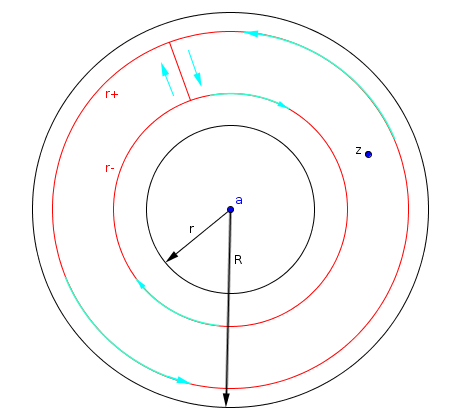
\includegraphics[width=0.4\textwidth]{immagini/teorema_laurent.png}
\end{figure}
Grazie alla formula integrale di Cauchy, sappiamo che  $\oint_C \frac{dz'}{2 \pi i} \frac{f(z')}{z-z'}$; possiamo vedere il cammino $C$ come somma di quattro cammini:
$$C=C(r+) \cup C(r-) \cup \text{ segmento percorso due volte in sensi opposti}$$
Si nota subito che il contributo del segmento è nullo, poichè viene percorso prima in un verso e poi nell'altro, e quindi i due contributi si annullano a vicenda. \\
Sostituendo tale cammino, l'integrale di Cauchy diventa:
$$\oint_{C(r+)} \frac{dz'}{2 \pi i} \frac{f(z')}{z-z'} - \oint_{C(r-)} \frac{dz'}{2 \pi i} \frac{f(z')}{z-z'}$$
dove il segno ''-'' davanti al secondo integrale mi permette di cambiare il verso di percorrenza della circonferenza $C(r-)$, in modo tale che entrambe le circonferenze siano percorse in senso antiorario.\\
Ora riscriviamo $\frac{1}{z-z'}$ come:
$$\frac{1}{(z'-a)-(z-a)}=\left\{  \begin{array}{l l}    \frac{1}{z'-a} \frac{1}{1-\frac{z-a}{z'-a}}=\sum_{l=0} ^{\infty} \frac{(z-a)^l}{(z'-a)^{l+1}} & \quad z' \in C(r+)\\    -\frac{1}{z-a} \frac{1}{1-\frac{z'-a}{z-a}}=-\sum_{l=0} ^{\infty} \frac{(z'-a)^l}{(z-a)^{l+1}} & \quad z' \in C(r-)  \end{array} \right.$$
Sostituiamo quindi gli sviluppi in serie geometrica negli integrali di prima e otteniamo:
$$f(z)=\oint_{C(r+)} \frac{dz'}{2 \pi i} f(z') \sum_{l=0} ^{\infty} \frac{(z-a)^l}{(z'-a)^{l+1}} - \oint_{C(r-)} \frac{dz'}{2 \pi i} f(z') \sum_{l=0} ^{\infty} \frac{(z'-a)^l}{(z-a)^{l+1}}=$$
$$=\sum_{l=0} ^{\infty} (z-a)^l \oint_{C(r+)} \frac{dz'}{2 \pi i} \frac{f(z')}{(z'-a)^{l+1}} - \sum_{l=0} ^{\infty} \frac{1}{(z-a)^{l+1}} \oint_{C(r-)} \frac{dz'}{2 \pi i} f(z') (z'-a)^l$$
dove abbiamo portato le sommatorie fuori dai rispettivi integrali poichè convergono uniformemente.\\
Dato che la funzione $f$ è olomorfa nell'anello $A$, possiamo sostituire i due cammini con altri cammini chiusi; oltretutto, dato che nell'integrale non compare $z$, tali cammini potranno attraversare quel punto. Otteniamo dunque che:
$$=\sum_{l=0} ^{\infty} (z-a)^l \oint_{\gamma} \frac{dz'}{2 \pi i} \frac{f(z')}{(z'-a)^{l+1}} - \sum_{l=0} ^{\infty} \frac{1}{(z-a)^{l+1}} \oint_{\gamma} \frac{dz'}{2 \pi i} f(z') (z'-a)^l$$
Cambiando indici nel secondo integrale (ponendo $m=l+1$), otteniamo lo sviluppo di Laurent.

Per quanto riguarda l'unicità, invece, supponiamo che esista un'altro sviluppo $\sum_{n=-\infty} ^{+\infty} \tilde{c_n} (z-a)^n$; mostriamo che $c_n=\tilde{c_n}$:
$$c_n= \oint_{\gamma} \frac{dz}{2 \pi i} \frac{f(z)}{(z-a)^{n+1}}= \oint_{\gamma} \frac{dz}{2 \pi i} \sum_{l=-\infty} ^{+\infty} \tilde{c_l} (z-a)^{l-n-1}= \footnote{Utilizziamo $l$ per indicare che stiamo guardando due sviluppi diversi.}$$
$$=\sum_{l=-\infty} ^{+\infty} \tilde{c_l} \oint_{\gamma} \frac{dz}{2 \pi i} (z-a)^{l-n-1}=\footnote{Ricordiamo che l'integrale vale 1 se $l-n-1=-1$, altrimenti è nullo} \sum_{l=-\infty} ^{+\infty} \tilde{c_l} \delta_{l-n-1,-1} = \tilde{c_n}$$

\end{proof}
Riportiamo alcuni esempi di sviluppi in serie di Laurent:
\begin{itemize}
\item Lo sviluppo in serie della funzione $f(z)=\frac{(z+1)^2}{z}$ è molto semplice da ottenere; infatti, basta  svolgere il quadrato al numeratore per ottenere tale sviluppo che risulta essere $z+2+\frac{1}{z}$, dove $z+2$ è la parte analitica mentre $\frac{1}{z}$ è la parte principale. Tale sviluppo in serie di Laurent è centrato in $z=0$ e vale sull'anello $0<z<\infty$; quando un anello è del tipo $0<z<a$, con $a>0$, viene detto \textbf{disco forato}.
%Nota: ricontrollare l'esempio qua sotto, perchè non sono sicuro sia giusto%
\item Sia data la funzione $f(z) = \frac{1}{z^2 (a-z)^2}$; dato che abbiamo due punti ''critici'', dobbiamo studiare le varie casistiche:
\begin{itemize}
\item Se $0<|z|<1$, possiamo scrivere uno sviluppo in serie di Laurent che convergerà nel disco forato centrato in $z=0$. Abbiamoche la funzione risulta essere:
$$\frac{1}{z^2} \frac{d}{dz} \left(\frac{1}{1-z} \right)=\footnote{Conosciamo il valore della somma della serie armonica semplice.} \frac{1}{z^2} \frac{d}{dz}(1+z+z^2+z^3+ \dots)= \frac{1}{z^2} \frac{d}{dz} \sum_{n=0} ^{\infty} z^n=$$
$$= \frac{1}{z^2} \sum_{n=0} ^{\infty} nz^{n-1}=\sum_{n=0} ^{\infty} nz^{n-3}=\frac{1}{z^2} + \frac{2}{z} + 3 + 4z + 5z^2 + \dots$$
dove la parte principale è $\frac{1}{z^2} + \frac{2}{z}$, mentre il resto compone la parte analitica.
\item Se invece andiamo a fare lo sviluppo di Laurent in $z=1$, avremo che in questo caso il disco di convergenza è $0<|z-1|<1$, cioè è il disco forato centrato in $z=1$. Otteniamo:
$$\frac{1}{z^2 (1-z)^2}=\frac{1}{(z-1)^2} \frac{1}{[1+(z-1)]^2}=\frac{1}{(z-1)^2} \sum_{n=0} ^{\infty} (-1)^n (z-1)^n=$$
$$= \frac{1}{(z-1)^2} \left(1-(z-1)+(z-1)^2-(z-1)^3+ \dots \right)=$$
$$=\frac{1}{(z-1)^2} - \frac{2}{(z-1)} + 3 - 4(z-1) + 5(z-1)^2 + \dots$$
dove la parte principale è $\frac{1}{(z-1)^2} - \frac{2}{(z-1)}$, mentre il resto forma la parte analitica.
\end{itemize}
\item Sia data la funzione $f(z)=e^{\frac{x}{2} (z- \frac{1}{z})}$; essa è una funzione olomorfa su $\C \backslash \{0\}$. Possiamo quindi sviluppare la funzione il serie di Laurent centrando tale sviluppo in $z=0$; otteniamo quindi uno sviluppo della forma:
$$\sum_{n=-\infty} ^{\infty} z^n J_n (x)$$
dove le $J_n(x)$ sono dette \textbf{funzioni di Bessel} con indice intero.
\end{itemize}
